\def\BibTeX{{\rm B\kern-.05em{\sc i\kern-.025em b}\kern-.08em
    T\kern-.1667em\lower.7ex\hbox{E}\kern-.125emX}}
% ASE2025
\documentclass[10pt,conference]{IEEEtran}

% \usepackage{cite}
\bibliographystyle{plainnat}
\usepackage[numbers]{natbib}
\usepackage{multirow}
\usepackage{enumitem}
\usepackage{balance}
\usepackage{tcolorbox}
\usepackage{graphicx}
\usepackage{amsmath}
\usepackage{hyperref}
\usepackage{pifont}
\usepackage{colortbl}
\usepackage{mdframed}
\usepackage{array}
\usepackage{tikz}
\usepackage{soul}
\usepackage{amsfonts}
\usepackage{tabularx}
\usepackage{makecell}
\usepackage{hhline}
\usepackage{float}

% add by yangdonghao
\usepackage{booktabs}

% add by aolangwoo
\usepackage{varwidth} 
\tcbuselibrary{breakable} 
\tcbuselibrary{skins} 
\usepackage{algorithm}
\usepackage{algorithmic}
% \usepackage[noend]{algpseudocode} %algorithm2e,algorithmic,
\usepackage{subcaption}
% \usepackage{subfigure}
% \newcolumntype{C}[1]{>{\centering\arraybackslash}p{#1}}
\newcommand{\xlian}[1]{\textcolor{blue}{\textbf{xlian}: #1}}
\newcommand{\mfk}[1]{\textcolor{purple!70!black}{\textbf{mfk}: #1}}

% 定义一个新环境
\newtcolorbox{ellipsebox}{
    enhanced,
    sharp corners,            % 如果不要尖角可改为 rounded corners
    frame style={draw=none},  % 先去掉矩形边框，后面用椭圆覆盖
    colback=gray!20,          % 浅灰背景（15% 灰度）
    colframe=gray!30,         % 边框颜色（稍深一点）
    arc=10pt,                  % 圆角半径（越大越接近椭圆）
    outer arc=10pt,
    boxrule=0.5pt,
    left=0pt, right=0pt, top=5pt, bottom=5pt,
    center,                   % 内容居中
    parbox=false,
    width=\linewidth,
    before skip=12pt, after skip=12pt,
    fontupper=\normalfont     % 取消粗体，使用正常字体
}


% summary环境
\newenvironment{rqsummary}[1]
{
    \vspace{2pt}
    \begin{mdframed}[
    linecolor=gray!100,
    linewidth=3pt,
    innerleftmargin=3pt,
    topline=false,
    rightline=false,
    bottomline=false,
    leftline=true,
    innerrightmargin=3pt,
    innertopmargin=3pt,
    innerbottommargin=3pt,
    backgroundcolor=gray!30
    ]
    \noindent\textbf{Summary for #1: }\ignorespaces
}
{
    \end{mdframed}
}

% set figure path
\graphicspath{{./figures/}} 

% Reduce spacing around floats
\setlength{\textfloatsep}{10pt plus 2pt minus 2pt}
\setlength{\floatsep}{10pt plus 2pt minus 2pt}
\setlength{\intextsep}{10pt plus 2pt minus 2pt}

%%
%% end of the preamble, start of the body of the document source.
\begin{document}

%%
%% The "title" command has an optional parameter,
%% allowing the author to define a "short title" to be used in page headers.
\title{Towards Pre-generation Requirement Uncertainty Assessment for Code Generation}
%\title{Mitigating Pre-generation Requirement Uncertainty for Reliable Code Generation}
%\title{Weak LLM-based Requirements Uncertainty Annotation for Pre-generation Taming for Reliable Code Generation}
%\title{\textsc{Clarify}: Mitigating Requirements Uncertainty before Code Generation}
\author{Anonymous Author(s)}

\maketitle

%%
%% The abstract is a short summary of the work to be presented in the
%% article.
\begin{abstract}
Large Language Models (LLMs) excel at code generation, but their performance is constrained by uncertainties in natural language requirements, such as ambiguity and under-specification. Existing workflows typically assess requirements uncertainty by comparing multiple generation outputs for the same requirement, a post-processing approach that tends to incur unnecessary time and resource consumption. This motivates a pre-generation solution that identifies and mitigates uncertainty beforehand, ensuring high-quality requirements are fed into the code generation process.
Thus, we introduce \textsc{Pulse} (Pre-generation Uncertainty Labeling with Surrogate Evaluator), a three-stage framework. First, we generate uncertain requirement variants via controlled perturbations and label uncertainty using a moderate-sized LLM oracle based on output variance across generations. Second, we train a lightweight RoBERTa-based classifier as a surrogate to predict uncertainty scores directly from textual features, avoiding generator invocation. Finally, we instantiate a simple agentic workflow that iteratively clarifies high-uncertainty requirements before generation. We evaluate \textsc{Pulse} on three functional-level benchmarks (HumanEval-ET, MBPP-ET, and LiveCodeBench) and further validate its generalizability on project-level code generation tasks (DevBench). Experimental results demonstrate four key findings. (1) Clarifying requirements identified as uncertain by \textsc{Pulse} improves pass@1 by up to 46\% and enhances generation stability across multiple runs. (2) Our proposed uncertainty quantification scores serve as an effective indicator, with higher requirements uncertainty correlating with greater pass@1 gains after clarification. (3) The lightweight classifier achieves high agreement with the oracle while incurring negligible inference overhead, making it suitable for real-time pre-generation screening. Finally, (4) \textsc{Pulse} generalizes well to project-level scenarios, confirming its practical utility beyond function-level benchmarks.

\end{abstract}

\begin{IEEEkeywords}
Code Generation;
Requirement Uncertainty;
Uncertainty Quantification;
Uncertainty Identification;
Uncertainty Clarification
\end{IEEEkeywords}

\section{Introduction}
\label{sec:intro}

% Requirement uncertainty exists and it effects generation reliability->background
Large Language Models (LLMs) have significantly advanced the state of automated code generation. Modern code generation systems are now capable of synthesizing executable programs in diverse programming languages from natural language requirements, achieving strong performance on widely adopted benchmarks such as HumanEval~\cite{humaneval}, MBPP~\cite{mbpp} and SWE-Bench~\cite{jimenez2024swebench}. Consequently, LLM-based code generation is being increasingly integrated into practical software engineering workflows through contemporary IDEs, serving a broad range of real-world development tasks across various sectors.

Despite these advances, the performance of LLM-based code generation still heavily depends on the quality of requirements. In real-world scenarios, requirements are often far from perfectly specified: they may contain vagueness, ambiguities, under-specification or implicit constraints~\cite{abdeahad2026accurate, ezzini2022anaphoric}. Such requirement-side imperfection may diverge the interpretations of code generation models, leading to requirements deviation in implementation, inconsistent outputs across different models, or instability across repeated generations, even when the underlying generation model is sufficiently capable~\cite{yang2026assessingimpactrequirementambiguity, 10554837}. In this work, we refer to these input-side deficiencies that cause unstable or low-quality code generation as \textit{requirements uncertainty}.

%Existing approaches identify it too late and too expensively,even we have clarifcation method such as clarifyGPT,it still use extra code genaration and tests...->existing method 
There is little doubt that requirement uncertainty poses a significant threat to the practical value of code intelligence.  Vijayvargiya et al.~\cite{vijayvargiya2026ambigsweinteractiveagentsovercome} reveal that AI models struggle to distinguish between well-specified and under-specified instructions, with the latter representing a common form of such uncertainty. In response, recent studies have begun to address requirement uncertainty through clarification or repair. For example, ClarifyGPT detects ambiguous requirements by generating test inputs and checking code consistency, before it asks targeted clarification questions~\cite{mu2024clarifygpt}. SpecFix repairs ambiguous problem descriptions by analyzing the distribution of programs induced by a requirement with testing and program repair techniques~\cite{jia2025specfix}. These studies provide valuable evidence that requirement uncertainty can be detected and mitigated.

However, these approaches rely on comparing consistency or distribution across multiple generation outputs, each of which is already resource-intensive. In modern code generation workflows that often involve planning, retrieval, generation, testing, iterative refinement~\cite{islam2024mapcoder,zhang2023repocoder, 11334685, zhao2025projectgen}, or multiple reasoning steps, this repeated execution cost is further multiplied. As a result, uncertainty is detected only after substantial resources have been expended across multiple runs, only to reveal that the root cause lies in the requirement itself. \emph{This motivates a lightweight pre-generation solution that assesses requirements uncertainty before any costly generation iteration is triggered.}

However, building such a solution is non-trivial.

\noindent \textbf{Challenge I: How to obtain reliable uncertainty signals for pre-generation use? }
Requirement uncertainty may arise from many forms of imperfect natural language descriptions, including ambiguity, vagueness, under-specification, implicit constraints, and even trivial noise~\cite{abdeahad2026accurate,ezzini2022anaphoric,yang2026assessingimpactrequirementambiguity}. However, not every textual imperfection necessarily harms code generation reliability. As modern LLMs become increasingly capable, some incomplete or implicit information may be inferred correctly, while seemingly minor textual variations may still lead to unstable implementations~\cite{chen2026nlperturbator}. Therefore, the key challenge is not merely to enumerate possible uncertainty types, but to obtain reliability-aware uncertainty signals that reflect whether a requirement is likely to cause unstable or low-quality code generation.

\noindent\textbf{Challenge II: How to predict requirement uncertainty before generation?} The demand of requirement uncertainty prediction before code generation makes post-generation approaches infeasible~\cite{mu2024clarifygpt, jia2025specfix}, due to the unavailability of execution results from generated code. While existing requirements ambiguity detection approaches often rely on human-labeled corpora~\cite{abdeahad2026accurate,ezzini2022anaphoric}, these methods originate from the requirements engineering community and are not tailored to code generation tasks. Our preliminary study shows that not all human-centric uncertainty uniformly transform into model-observed uncertainty.  Hence, their ambiguity labels do not directly indicate whether a requirement will lead to unreliable generation. In contrast, reliability-aware uncertainty is inherently tied to the model's generation behavior, specifically, the correctness and consistency of its outputs. Since neither the generated programs nor their execution feedback is accessible prior to generation, a practical solution must predict such uncertainty directly from the requirement text, while also implicitly taking the model's responses into account.

% \noindent\textbf{Challenge III: How to use uncertainty to guide clarification automatically and effectively?}
% Even if requirement uncertainty can be identified before generation, mitigating it automatically remains non-trivial. A natural way to reduce uncertainty is to ask targeted clarification questions and rewrite the requirement based on the received responses, as adopted by clarification-based code generation frameworks~\cite{mu2024clarifygpt}. However, effective clarification requires more than simply asking additional questions. Prior work shows that directly prompting LLMs to detect and resolve ambiguous requirements may produce irrelevant or inconsistent clarifications~\cite{jia2025specfix}. Therefore, the key challenge is how to leverage the quantified uncertainty signals to ask pertinent clarification questions and automatically rewrite the requirement based on the clarification responses, so that the clarified requirement genuinely reduces uncertainty rather than introducing redundant or misleading details.

To address the above challenges, we propose our approach \textsc{Pulse} (Pre-generation Uncertainty Labeling with Surrogate Evaluator). It includes three stages. Firstly, we inject the perturbations mentioned in literature into the requirements description of public benchmarks, and labeling the uncertainty based on the multiple execution of a moderate-size code generation model. Second, with the annotated dataset, we train a lightweight RoBERTa-based classifier as a surrogate model to directly predict uncertainty scores from surface textual features. The classifier categorizes requirements into two uncertainty levels (high- and low- risk) with low inference overhead, enabling practical pre-generation risk assessment.  The high-risk results trigger the downstream clarification process. Third, we instantiate a simple agentic workflow that adopts an asking-answering pattern to iteratively clarify high-uncertainty requirements before generation takes place.

We construct our training dataset from three standalone functional benchmarks, HumanEval-ET~\cite{humaneval}, MBPP-ET~\cite{mbpp}, and LiveCodeBench~\cite{jain2025livecodebench}, and train our classifier on it. On functional-level benchmarks with four generation approaches (two LLMs and two state-of-the-art frameworks), our experiments demonstrate: (1)  the effectiveness of \textsc{Pulse} in improving both pass@1 (by up to 46\%) and stability when requirements are clarified prior to generation; (2) the utility of our proposed uncertainty quantification (UQ) as a signal for requirement clarification, with higher UQ scores correlating with greater post-clarification gains; (3) the efficiency of our lightweight classifier. In addition, we validate the generalizability of our approach on project-level code generation tasks using a public benchmark that consists of 10 real-world repositories.

%train a lightweight classifier to predict requirement uncertainty directly from requirement text. We evaluate \textsc{Pulse} primarily on function-level code generation, and additionally conduct a preliminary project-level study to examine its applicability beyond standalone tasks. The results show that uncertainty-aware selective clarification improves pass@1 across most function-level settings and remains compatible with both direct LLM generation and representative generation-time baselines.



% latex problem -- this table should be displayed near the section Prestudy
\begin{table*}[htbp]
\centering
\caption{Requirement perturbations used in the preliminary study. These perturbations are adapted from prior studies on natural-language perturbation and prompt robustness.}
\label{tab:uncertainty_factors}
\begin{tabular*}{\textwidth}{@{\extracolsep{\fill}}p{3.3cm}p{8.0cm}p{3.0cm}p{2.0cm}@{}}
\toprule
\textbf{Perturbation Type} & \textbf{Explanation} & \textbf{Transformation Method} & \textbf{Reference} \\
\midrule

Content Rewriting
& Rewrite the requirement by abstracting or paraphrasing detailed expressions of functional constraints, edge cases, or task intent while keeping the same high-level programming task.
& LLM-assisted rewriting
& ~\cite{chen2026nlperturbator,zhu2024promptrobust} \\

Format Transformation
& Rewrite the requirement into a natural, conversational, and human-like paragraph, avoiding formal benchmark-style structures while preserving all functional requirements and constraints.
& LLM-assisted rewriting
& ~\cite{chen2026nlperturbator} \\

Example Removal
& Remove input-output examples from the requirement, such as doctest-style example usages in HumanEval and sample input/output cases in programming-contest-style tasks such as LiveCodeBench.
& Rule-based removal
& ~\cite{nashid2023retrieval,khojah2025impact} \\

Verbose Rewriting
& Add redundant descriptions or expand the requirement expression while preserving the intended functionality.
& Rule-based transformation
& ~\cite{chen2026nlperturbator,zhu2024promptrobust} \\

Noise Injection
& Insert irrelevant or distracting natural-language content into the requirement without introducing new inputs, outputs, constraints, or expected behavior.
& Rule-based transformation
& ~\cite{chen2026nlperturbator,zhu2024promptrobust} \\

Typographical Perturbation
& Introduce spelling or character-level errors while aiming to preserve the original requirement intent.
& TextAttack-based character transformation
& ~\cite{morris2020textattack,zhu2024promptrobust} \\

\bottomrule
\end{tabular*}
\end{table*}



In summary, the contributions of this paper are threefold:
\begin{itemize}[leftmargin=1em]

    \item \textbf{Approach.} We propose \textsc{Purse}, a novel framework for assessing requirement uncertainty without executing code generation. It serves as a lightweight, plug-and-play guardrail that can be seamlessly integrated with existing requirements clarification methods and code generation pipelines.
    
    \item \textbf{Labeling.} To address the scarcity of uncertainty-aware requirement datasets for reliable code generation, we propose a labeling method that annotates requirement uncertainty via execution feedback from a moderate-size code generation model, facilitating benchmark construction for both  classifier training and evaluation purposes.

    \item \textbf{Evaluation.} Extensive experiments on four public benchmarks demonstrate the effectiveness of our \textsc{Purse} and its classifier, as well as its good generalization to project-level code generation tasks. The source code and data are publicly available at  \url{https://figshare.com/s/bb1ffe8ca97f6ab5ab95}.
    % \item We introduce a model-centered definition of requirement uncertainty for code generation and characterize uncertainty through generation consistency under repeated sampling.
    % \item We propose a consistency-based uncertainty quantification method combining pass-rate entropy and CodeBLEU-based generation divergence.
    % \item We develop a lightweight requirement uncertainty classifier that enables pre-generation uncertainty prediction directly from requirement text.
    % \item We design an uncertainty-aware selective clarification framework and demonstrate its effectiveness in both function-level and repository-level code generation tasks.
\end{itemize}


\section{Preliminary Study}
\label{sec:preStudy}

% Motivation and study questions
Existing studies have shown that ambiguous, noisy, or incomplete requirements can degrade the performance of code generation models~\cite{vijayvargiya2026ambigsweinteractiveagentsovercome,10554837,mu2024clarifygpt,jia2025specfix}. While several studies have investigated the impact of various uncertainty factors, such as clarity, typographical errors, and the presence or absence of examples~\cite{10.1145/3697010,liu2024trustworthyllmssurveyguideline,DBLP:journals/corr/abs-2406-10101,xia-etal-2025-survey}, their primary evaluation metric has been the test-case passing rate. In this preliminary study, we aim to explore how these factors affect the reliability of code generation.

%Perturbation design and dataset construction
\noindent\textbf{Study Setup.} Our preliminary study follows a three-step pipeline. We first collect perturbation types from prior studies on natural-language perturbation, prompt robustness, and requirements ambiguity, as summarized in Table~\ref{tab:uncertainty_factors}. We then inject these perturbations into the requirement descriptions of public benchmarks to construct perturbed inputs. Finally, we evaluate the quality and stability of generated code under these perturbed requirements. Specifically, we use HumanEval-ET, the extended-test version of HumanEval from EvalPlus~\cite{humaneval,liu2023evalplus}, as a controlled function-level testbed. We further include LiveCodeBench~\cite{jain2025livecodebench} as a more challenging benchmark to examine whether the observed effects generalize beyond HumanEval-style prompts.

%explain the purbation types
Referring to the existing literature, the perturbation process combines LLM-assisted rewriting, rule-based transformation, and TextAttack-based character transformation~\cite{morris2020textattack}. Specifically, content rewriting and format transformation are generated through LLM-assisted rewriting, where they require preserving the original task intent while changing the semantic expression or presentation style of the requirement. For content rewriting, the LLM is prompted to paraphrase or abstract detailed expressions of functional constraints, edge cases, or task intent. For format transformation, the LLM rewrites the requirement into a more natural and conversational paragraph while preserving the original functional requirements and constraints. Example removal, verbose rewriting, and noise injection are implemented using rule-based transformations. Example removal deletes input-output examples from the original prompt, such as doctest-style examples in HumanEval-style tasks and sample input-output cases in programming-contest-style tasks. Verbose rewriting adds redundant explanatory descriptions, while noise injection appends task-irrelevant natural-language sentences that do not introduce new inputs, outputs, constraints, or expected behaviors. Typographical perturbation is generated using TextAttack-based character transformations that introduce spelling or character-level errors while preserving the readability of the requirement. %After transformation, we manually inspect the perturbed requirements to ensure that they remain readable, preserve the intended programming task, and match the intended perturbation type.\mfk{maybe can add some examples here and simplify the discussion accordingly} \xlian{Human checking on all cases?}

% \xlian{if possible to merge the generation process? Most of them need prompting LLM. You can first describe explicitly} The perturbation process combines LLM-assisted transformation, deterministic rules, and character perturbations based on TextAttack, a Python framework for adversarial attacks and data augmentation in NLP ~\cite{morris2020textattack}. \xlian{update this paragraph according to the type in Table} For content perturbations, LLM-based content rewriting is generated by prompting the LLM to rephrase the requirement while preserving the intended functionality, whereas example removal is performed by deterministically removing the input-output examples provided in the original benchmark prompt, such as example usages and expected outputs \xlian{ambiguity: example usage}in HumanEval-style task descriptions\cite{humaneval}. Structural perturbations are generated through LLM-assisted format transformation, where the LLM is prompted to reorganize the requirement presentation, such as\xlian{or including?} changing line breaks\xlian{what is this?}, ordering, or layout\xlian{what is line layout? Can give examples}, without intentionally modifying the target functionality\xlian{without modifying the intention?}. We use LLM-assisted formatting because requirement prompts from different benchmarks, and even prompts within the same benchmark, often vary substantially in organization, making fixed formatting rules difficult to apply consistently. Expressive perturbations, including verbose expansion and noise injection, are produced using simple rule-based procedures, such as adding redundant descriptions or appending irrelevant distracting sentences \xlian{what is the irrelevant sentences? how do you select?} without intentionally changing the target functionality. Character perturbations are generated using TextAttack-based transformations\cite{morris2020textattack} that introduce typographical or character-level errors while largely preserving the original intent. After transformation, \xlian{we get XX perturbed requirements.} we manually inspect the them to ensure that they remain readable, preserve the intended task where applicable, and correspond to the intended perturbation family.

We conduct code generation experiments using DeepSeek-v4-flash~\cite{deepseekai2026deepseekv4}, a strong instruction-following code generation model. We choose a capable model because the preliminary study aims to examine whether common requirement-side perturbations can still affect generation reliability under a strong code generation setting. For each original or perturbed requirement, we sample the model $K$ times under the same decoding configuration and execute the generated programs against the corresponding test cases. We report both the test-case passing rate and generation inconsistency across repeated samples, allowing us to analyze not only whether the generated programs are functionally correct, but also whether the model produces stable solutions for the same requirement.

%latex problem -- this figure should be displayed at the next page of the table 1
\begin{figure*}[t]
\centering
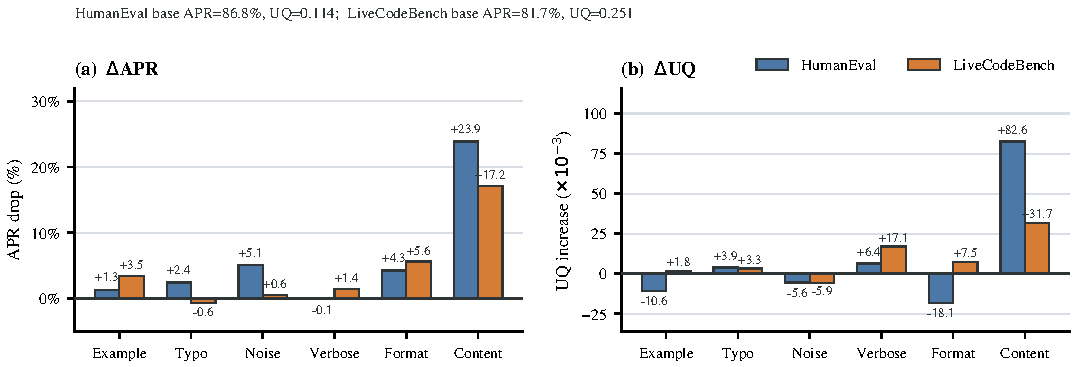
\includegraphics[width=1\textwidth]{preliminary_study_overview.pdf}
\caption{Impact of six requirement perturbation types on average pass-rate (APR) degradation and model-observed uncertainty (UQ) increase. $\Delta APR$ is computed as $APR_{\mathrm{orig}}-APR_{\mathrm{pert}}$ and $\Delta UQ$ is computed as $UQ_{\mathrm{pert}}-UQ_{\mathrm{orig}}$.}
\label{fig:preliminary-study-overview}
\end{figure*}

%explain the metric
\noindent \textbf{Metrics.} In this preliminary study, we set $K=5$ for repeated sampling. We evaluate code generation reliability using two complementary metrics: average pass rate, denoted as $APR$, and uncertainty quantification score, denoted as $UQ$. Our measurement of requirement uncertainty via code execution rests on a key assumption: since requirement uncertainty is not directly observable, we adopt generation inconsistency across repeated samples as a model-observed proxy. This assumption aligns with the existing work~\cite{mu2024clarifygpt, jia2025specfix}. 

Our intuition about uncertainty quantification is that an uncertain requirement may lead the model to generate programs that differ in implementation structure or behave inconsistently under the test suite. Accordingly, we consider two signals of generation inconsistency: structural inconsistency, which captures pairwise differences in generated code measured by CodeBLEU distance~\cite{ren2020codebleu}, and functional inconsistency, which captures variation in test execution outcomes across repeated samples.
We merge the metrics of these two views here to enhance comprehensiveness. 

Let $r_i$ denote the $i$-th requirement and $g_{ij}$ denote the $j$-th program generated for $r_i$ under repeated sampling, where $j\in{1,\ldots,K}$. We execute $g_{ij}$ against the corresponding test suite and define $t_{ij}\in[0,1]$ as the fraction of test cases passed. We compute the average pass rate of requirement $r_i$ as:
\begin{equation}
\label{eq:avgPassRate}
APR(r_i)=\frac{1}{K}\sum_{j=1}^{K}t_{ij}
\end{equation}
At the benchmark level, we report the mean $APR$ over all evaluated requirements, i.e., $\frac{1}{N}\sum_{i=1}^{N}APR(r_i)$.

While $APR(r_i)$ measures average functional correctness, it does not capture whether repeated generations implement the same requirement in structurally different ways. Therefore, we measure structural inconsistency using the average pairwise CodeBLEU distance among generated programs~\cite{ren2020codebleu}:
\begin{equation}
\label{eq:codebleuDistance}
D(r_i)=\frac{2}{K(K-1)}\sum_{1\leq a<b\leq K}
\left(1-\mathrm{CodeBLEU}(g_{ia},g_{ib})\right)
\end{equation}
A higher $D(r_i)$ indicates that repeated generations produce implementations with greater structural inconsistency for the same requirement.

However, structural inconsistency alone does not indicate whether the generated programs behave consistently under the test suite. Therefore, we further use the variation of test-case passing rates as an observable signal of functional inconsistency. Let $T_i={t_{i1},t_{i2},\ldots,t_{iK}}$ denote the set of passing rates observed under requirement $r_i$. We compute the variance of $T_i$ as:
\begin{equation}
\label{rq：passRateVariance}
\mathrm{Var}(T_i)=\frac{1}{K}\sum_{j=1}^{K}\left(t_{ij}-APR(r_i)\right)^2
\end{equation}
The functional inconsistency observed under $r_i$ is then defined as the normalized variance:
\begin{equation}
\label{eq:functionalInconsistency}
S(r_i)=\min\left(\frac{\mathrm{Var}(T_i)}{0.25}, 1\right)
\end{equation}
Since each $t_{ij}$ is bounded in $[0,1]$, we use the Bhatia--Davis inequality to bound the variance of the empirical passing-rate distribution~\cite{bhatia2000better}. Let $\mu_i=APR(r_i)$ denote the mean passing rate. The inequality gives
$$
\mathrm{Var}(T_i)\leq(1-\mu_i)(\mu_i-0)
=APR(r_i)(1-APR(r_i)).
$$
Since $APR(r_i)(1-APR(r_i))$ is maximized at $APR(r_i)=0.5$, we have $\mathrm{Var}(T_i)\leq0.25$. We therefore use $0.25$ as the normalization constant.


Finally, we compute the uncertainty score of requirement $r_i$ by equally combining structural and functional inconsistency:
\begin{equation}
\label{eq:uq}
UQ(r_i)=\frac{1}{2}\left(D(r_i)+S(r_i)\right)
\end{equation}
We report $APR$ separately as the correctness metric; therefore, $UQ$ focuses on generation inconsistency rather than directly incorporating average correctness. A larger $UQ$ value indicates higher model-observed requirement uncertainty.

Figure~\ref{fig:preliminary-study-overview} reports the impact of requirement perturbations on both HumanEval-ET and LiveCodeBench using the original requirements as the reference point. For each perturbation type, we report two relative metrics: average pass-rate degradation and uncertainty increase. Specifically, the former is computed as $\Delta APR=APR_{\mathrm{orig}}-APR_{\mathrm{pert}}$, where a positive value indicates that the perturbation reduces functional correctness. And the latter is computed as $\Delta UQ=UQ_{\mathrm{pert}}-UQ_{\mathrm{orig}}$, where a positive value indicates that the perturbation increases model-observed requirement uncertainty.


\begin{ellipsebox}
\centering
\normalfont\itshape
\textbf{Observation: Human-perceived perturbations do not uniformly translate into model-observed uncertainty.}
\end{ellipsebox}

Several surface-level perturbations have limited or inconsistent effects across benchmarks. For example, typographical perturbation leads to only a small increase in $UQ$ on both HumanEval-ET and LiveCodeBench, while noise injection even decreases $UQ$ in both settings. Verbose rewriting shows benchmark-dependent effects: it has almost no pass-rate impact on HumanEval-ET, but causes a clearer pass-rate drop and uncertainty increase on LiveCodeBench. These results suggest that perturbations that appear noisy or verbose from a human perspective are not necessarily the main source of model-observed uncertainty.

In contrast, content rewriting consistently causes the strongest degradation across both benchmarks. It leads to the largest $\Delta APR$ on HumanEval-ET and LiveCodeBench, and also produces the largest increase in $UQ$ on both datasets. This indicates that perturbations affecting the semantic expression of functional constraints, edge cases, or task intent are more likely to induce observable degradation and generation inconsistency than surface-level noise alone. Format transformation also shows non-negligible impact, especially in terms of pass-rate degradation, but its effect on $UQ$ is less consistent across benchmarks.

This observation carries an important implication for our study: requirement uncertainty should not be defined by whether a requirement appears ambiguous, noisy, or perturbed from a human perspective. Some perturbations that seem problematic to humans can be handled robustly by a strong code generation model, while others can induce clear correctness degradation or generation inconsistency. Therefore, in the following sections, we explore two directions: (1) how to annotate requirement uncertainty in a way that impact reliable code generation, and (2) how to proactively identify such uncertainty before code generation.


\section{Our Approach}
\label{sec:approach}

% latex problem -- this figure should be displayed near the section approach
\begin{figure*}[t]
  \centering
  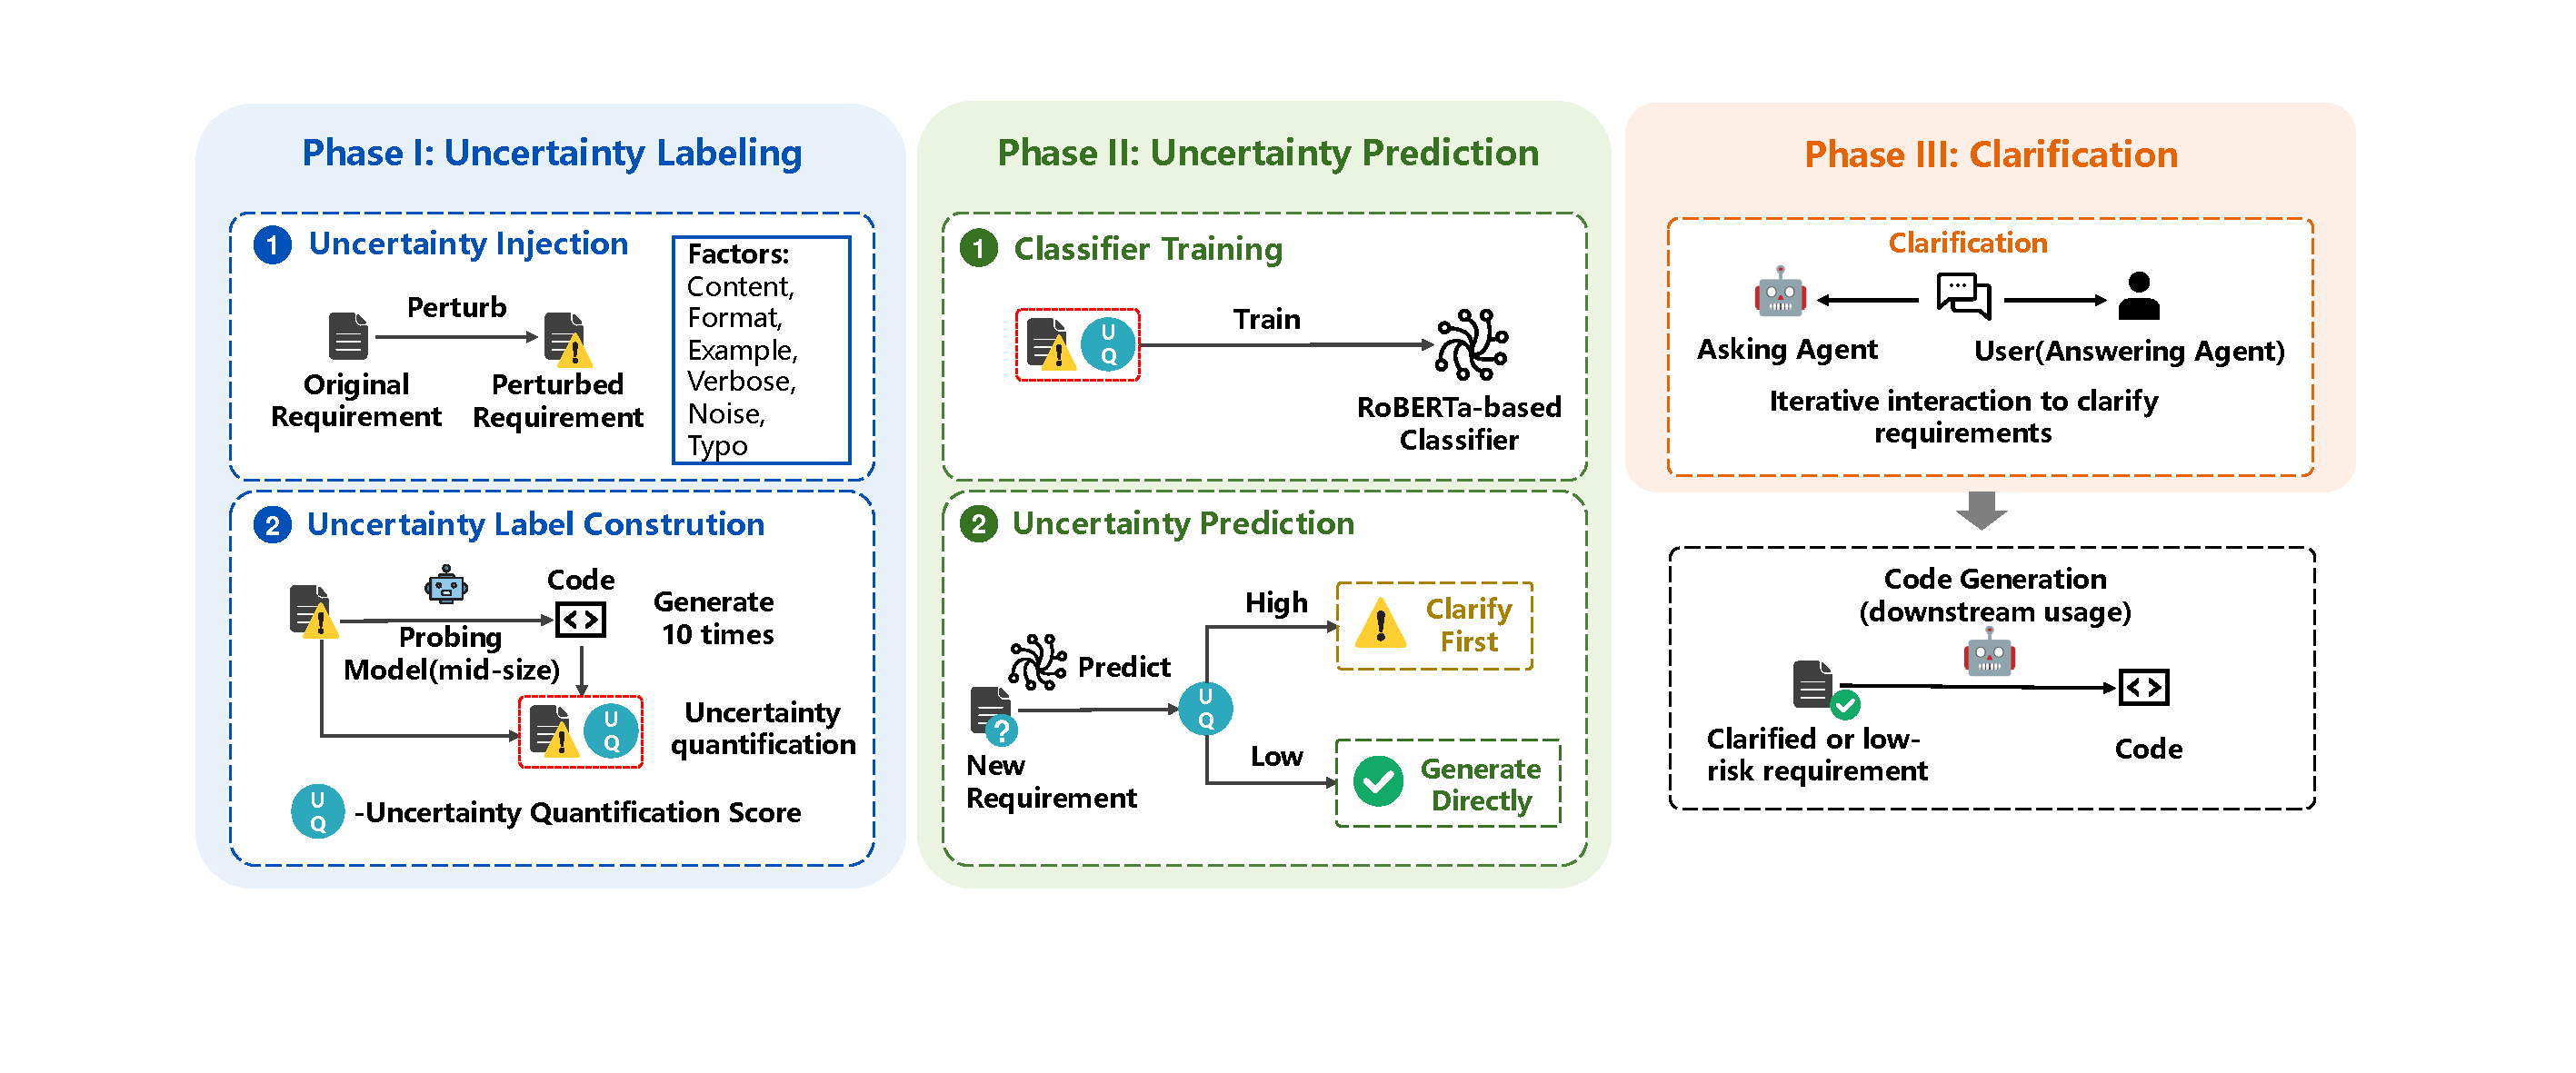
\includegraphics[trim={2cm, 3.5cm, 4.5cm, 1.5cm}, clip, width=0.95\textwidth]{overview.pdf}
  \caption{Overview of our approach \textsc{Pulse}.}
  \label{fig:approach-figure}
\end{figure*}

Figure~\ref{fig:approach-figure} illustrates the workflow of our approach, \textsc{Pulse}, which consists of three stages: requirement uncertainty labeling, requirement uncertainty prediction, and uncertainty-aware clarification. In Stage I, we inject perturbation types that affect code generation reliability (see Section~\ref{sec:preStudy}) into benchmark requirements. Inspired by Expert-Novice Differences~\cite{Chi1981ExpertNovice} and schema-theoretic default reasoning~\cite{Rumelhart1980Schemata}, we use a moderate-sized model, Qwen2.5-7B-Coder-Instruct, to annotate requirements prone to unreliable generation, following the uncertainty metric in Section~\ref{sec:preStudy}. In Stage II, the resulting $UQ$ scores are transformed into binary labels to train a lightweight RoBERTa-based classifier. Given a requirement, the classifier estimates the probability that the requirement belongs to the high-uncertainty class, thereby enabling efficient pre-generation assessment without repeated generation. In Stage III, the predicted uncertainty label drives intervention: uncertainty-prone requirements undergo clarification before generation, while low-risk ones proceed directly. To enable scalable evaluation, we implement a multi-agent simulation of clarification dialogues between a code generator and a user.

\subsection{Requirement Uncertainty Labeling}

We adopt the uncertainty injection setup from Section~\ref{sec:preStudy}. This section then details the selection of the probe model and the UQ-based binary labeling process.

\subsubsection{Uncertainty Probe Model}

Requirement uncertainty labeling relies on repeated generation to observe whether a requirement induces stable or unstable high-quality code generation outcomes. Since our goal is to label uncertainty that can lead to unreliable code generation across multiple runs and models, the choice of the generator model is critical: different models may exhibit different sensitivity to the same requirement perturbation, and the label should largely reflect model-agnostic uncertainty.

We use a moderate-sized code generation model as the uncertainty probe. According to Expert-Novice Differences~\cite{Chi1981ExpertNovice} and schema-theoretic default reasoning~\cite{Rumelhart1980Schemata}, we reason that frontier models tend to automatically clarify uncertain requirements. As a result, they compress both functional instability and structural divergence, making requirements that appear clear to expert models potentially uncertain for other models. In contrast, a moderate-sized model retains good capability in requirement interpretation while being more sensitive to requirement variations. 

We empirically verify this reasoning with a simple evaluation. Table~\ref{tab:model_selection} compares generation reliability and uncertainty across models of different capacities. On HumanEval-ET, DeepSeek-V3.2 achieves a slightly higher APR than Qwen2.5-7B-Coder-Instruct\cite{hui2024qwen2.5} while producing a much smaller mean UQ score. Similar trends can also be observed on MBPP-ET. These results suggest that stronger models may mask requirement-induced uncertainty through more stable generation, whereas a moderate-sized model can better expose variation in generation consistency. Therefore, we use Qwen2.5-7B-Coder-Instruct as the uncertainty probe for constructing UQ-based labels.

\begin{table}[t]
\vspace{0.5em}
\centering
\caption{Effect of model capacity on generation reliability and uncertainty. APR denotes Average Pass Rate and UQ denotes Mean Uncertainty Score.}
\label{tab:model_selection}
\footnotesize
\setlength{\tabcolsep}{4pt}
\begin{tabular*}{\columnwidth}{@{\extracolsep{\fill}}llll@{}}
\hline
Dataset & Model & APR & UQ \\
\hline
HumanEval-ET & DeepSeek-V3.2 & 0.844 & 0.057 \\
HumanEval-ET & Qwen2.5-7B-Coder-Instruct & 0.807 & 0.154 \\
MBPP-ET & DeepSeek-V3.2 & 0.527 & 0.148 \\
MBPP-ET & Qwen2.5-7B-Coder-Instruct & 0.493 & 0.255 \\
\hline
\end{tabular*}
\end{table}

\subsubsection{UQ-based Binary Labeling}

Following the UQ metric defined in Section~\ref{sec:preStudy}, we assign each requirement instance a model-centered uncertainty score based on repeated generation inconsistency. Specifically, for each requirement $r$, we repeatedly sample $K=10$ generated programs from the uncertainty probe model and evaluate them against the corresponding test suite. The resulting UQ score summarizes the degree to which repeated generations are inconsistent in terms of functional outcomes and implementation structures.

To support requirement uncertainty prediction, we need binary supervision labels indicating whether a requirement should be treated as high-uncertainty. While Stage I produces a continuous UQ score instead of a discrete class label. To obtain supervision for classifier training, we convert the continuous UQ score into a binary label using a two-component Gaussian Mixture Model (GMM)~\cite{bishop2006pattern}. Instead of applying a manually fixed threshold to the continuous UQ scores, we use GMM to derive data-driven labels based on the empirical distribution of UQ scores. This makes our label construction less dependent on hand-tuned thresholds and, more importantly, allows our method to automatically adapt to different datasets without requiring dataset-specific calibration. GMM-based soft grouping has also been adopted in recent uncertainty quantification studies to model latent structures in generated outputs~\cite{luo2026agsc}.

In our setting, each requirement $r$ is associated with a continuous uncertainty score $U(r)$ computed in Stage I. The GMM treats the distribution of $U(r)$ as a mixture of two latent components, corresponding to low-risk and high-uncertainty requirements. We fit the GMM using the classical EM algorithm~\cite{dempster1977maximum}. After fitting the mixture model, we assign the component with the larger mean UQ score to the high-uncertainty class. Let $z$ denote the latent component assignment and let $z=1$ represent the high-uncertainty component. We then define the binary uncertainty label $y(r)$ according to the GMM posterior probability:
\begin{equation}
\label{eq:gmmLabel}
y(r)=
\begin{cases}
1, & P_{\mathrm{GMM}}(z=1 \mid U(r)) \geq 0.5,\\
0, & P_{\mathrm{GMM}}(z=1 \mid U(r)) < 0.5,
\end{cases}
\end{equation}
where $P_{\mathrm{GMM}}(z=1 \mid U(r))$ denotes the posterior probability estimated by the fitted GMM. This probability is used only for label construction, whereas the classifier later predicts $p(y=1\mid r)$ directly from the requirement text.

The resulting binary labels serve as supervision signals for training the requirement uncertainty classifier in Stage II. In this way, repeated generation is only used offline to construct model-centered labels, while the trained classifier enables direct uncertainty assessment from requirement text at inference time.

\subsection{Requirement Uncertainty Prediction}

%Requirement uncertainty labeling provides model-centered supervision signals for identifying requirements that are likely to induce unreliable generation. However, computing UQ scores requires repeated code generation and test execution, which is costly for pre-generation assessment. 
We train a lightweight classifier that estimates requirement uncertainty directly from requirement text.


\subsubsection{Problem Formulation}
Given a natural language requirement $r$, our objective is to predict whether it belongs to the high-uncertainty class without performing repeated code generation. Based on the binary labels $y(r)$ constructed above, we train an uncertainty prediction model $f(\cdot)$ that maps $r$ to the probability of the high-uncertainty class:
\begin{equation}
\label{eq:uncertaintyPrediction}
f(r) \rightarrow p(y=1 \mid r),
\end{equation}
where $p(y=1 \mid r)$ denotes the classifier-predicted probability that requirement $r$ belongs to the high-uncertainty class. Since the classifier output is a continuous probability, it must be converted into a binary decision before being used as a clarification trigger. A fixed threshold of $0.5$ assumes that classifier scores are well calibrated and that the two classes have balanced decision costs, which may not hold in our setting. In particular, high-uncertainty requirements are the primary targets for clarification, and missing such cases may prevent potentially beneficial clarification from being triggered. Therefore, following threshold-selection practice for optimizing classification decisions~\cite{lipton2014optimal}, we select a decision threshold $\tau$ on the validation set and choose the threshold that maximizes the validation objective for identifying high-uncertainty requirements. The resulting binary prediction is defined as:
\begin{equation}
\label{eq:predictionLabel}
\hat{y}(r)=
\begin{cases}
1, & p(y=1 \mid r) \geq \tau,\\
0, & p(y=1 \mid r) < \tau,
\end{cases}
\end{equation}
where $\hat{y}(r)=1$ indicates that the requirement is predicted as high-uncertainty and should trigger uncertainty-aware clarification, while $\hat{y}(r)=0$ indicates that the requirement is treated as low-risk.


\subsubsection{Classifier Training}
%To enable efficient requirement uncertainty prediction, 
We adopt RoBERTa~\cite{liu2019roberta} as the backbone text encoder and attach a lightweight binary classification head. 
We select RoBERTa because it provides strong contextual text representations for natural language understanding tasks while remaining substantially more lightweight than generation models, making it suitable for efficient pre-generation uncertainty prediction~\cite{liu2019roberta,devlin2019bert}. 
Given a requirement description, the encoder maps the input text into contextualized representations, which are then passed to the classification head to estimate the probability that the requirement belongs to the high-uncertainty class.
The trained classifier enables the determination of whether a given requirement description exhibits uncertainty.


\subsection{Uncertainty-aware Clarification}
Requirements with high uncertainty are flagged for clarification, while low-risk ones are directly used for code generation. The clarification itself can be handled by external methods. In this work, inspired by human–AI interaction, we design a simple multi-agent clarification framework (Figure~\ref{fig:approach-figure}). It consists of an asking agent that initiates clarification questions and an answering agent that simulates user responses.

The asking agent targets issues that may undermine reliable code generation, such as ambiguity, underspecification, inconsistency, and missing constraints. To keep questions actionable, it focuses on implementation-relevant details like edge cases, I/O types, error handling, performance, and missing context, rather than posing generic queries.

To control cost, the process is bounded by a maximum number of rounds and can terminate early when further dialogue yields no actionable information. After the ask–answer loop, \textsc{Pulse} consolidates the confirmed information into a clarified requirement. Instead of rewriting, we keep the original requirement as the main specification and attach each clarification in the form of \emph{[original requirement] + [1. clarified info] + [2. clarified info] + ....} This provenance-aware formulation is inspired by prior work that refines ambiguous requirements based on additional evidence rather than arbitrary rewriting~\cite{mu2024clarifygpt,jia2025specfix}, helping avoid semantic drift while still making implicit details explicit for downstream code generation.

\section{Experimental Setup}\label{sec:setup}



We evaluate our \textsc{Pulse} by addressing the following four research questions (RQ).
\begin{itemize}[leftmargin=1em]
\item \textbf{RQ1: Overall Effectiveness.}
To what extent does requirement clarification with \textsc{Pulse} improve the performance of function-level code generation?
\item \textbf{RQ2: Uncertainty Quantification.}
To what extent can our proposed uncertainty quantification serve as effective signals for requirement clarification?
\item \textbf{RQ3: Uncertainty Prediction.}
Does our lightweight classifier outperform LLM-based uncertainty assessment?
\item \textbf{RQ4: Generalization.}
To what extent can our \textsc{Pulse} trained on function-level datasets generalize to project-level code generation scenarios?
\end{itemize}



\subsection{Datasets}
For RQ1--RQ3, we use three widely used function-level code generation benchmarks: HumanEval-ET~\cite{humaneval}, MBPP-ET~\cite{mbpp}, and LiveCodeBench~\cite{jain2025livecodebench}. HumanEval-ET includes 164 hand-crafted problems with rigorous test cases, offering high-quality evaluation at a small scale. MBPP-ET comprises 974 crowd-sourced basic Python tasks, providing broader coverage of everyday programming constructs. LiveCodeBench contains competitively sourced programming problems with temporal annotations, enabling time-aware evaluation. 

For LiveCodeBench\footnote{\url{https://github.com/LiveCodeBench/LiveCodeBench}}, we follow the official GitHub repository and use \texttt{release\_v6}, the latest listed cumulative snapshot of the code-generation-lite scenario at the time of our experiments. This release contains 1,055 problems collected from May 2023 to April 2025. To align LiveCodeBench with our function-level evaluation protocol, we retain only problems with explicit function signatures, resulting in 444 tasks. This ensures that all three benchmarks follow a consistent function-level generation and pass/fail testing protocol.


For RQ4, to evaluate whether \textsc{Pulse} generalizes beyond standalone function-level generation, we adopt the project-level evaluation setup from ProjectGen~\cite{zhao2025projectgen} and use the benchmark of DevBench$_{Python}$ ~\cite{li2025devbench}, the Python subset of DevBench.  It comprises 10 small-scale project-level tasks with executable tests, averaging 2.2 files and 276 lines of code per task. Although small in scale, these tasks involve project-level logic across multiple files, functions, and tests.


\subsection{Baselines and Implementation Details}
To assess the impact of requirement clarification via \textsc{Pulse}, we evaluate its effectiveness on two advanced LLMs accessed through APIs: DeepSeek-V4-Flash (DeepSeek)~\cite{deepseekai2026deepseekv4} and GPT-5.4-mini (GPT)~\cite{openai2026gpt54system}, and two representative strong code generation baselines, MapCoder~\cite{islam2024mapcoder} and DebateCoder~\cite{chen2025debatecoder}. MapCoder improves code generation through multi-agent collaborative reasoning and iterative refinement, while DebateCoder enhances generation reliability by introducing a debate-style interaction among multiple coding agents.

In the clarification phase, to mitigate human variability, we use the same LLM as the asking agent to serve as the answering agent, simulating human respondents with access to the ground-truth intent. Specifically, the answering agent responds to clarification questions based solely on the original requirements and is instructed to provide only minimal and direct answers to the given questions. This design ensures that the clarification process exposes only task-relevant intent information, rather than unnecessary answer leakage.

We split each dataset of function-level benchmarks into training, validation, and testing subsets with a 6:2:2 ratio. The training subset is used to construct uncertainty labels and train the uncertainty classifier, the validation subset is used for threshold tuning, and the testing subset is held out for final evaluation. We combine the training datasets of the three benchmarks into a single corpus for classifier training, allowing the classifier to be trained once and then applied across different benchmarks. During addressing RQ1-RQ3, we report performance both on the full testing subset and on the clarified subset selected by the uncertainty classifier, so as to distinguish overall effectiveness from the effect on requirements that actually undergo clarification.
\section{Results and Analysis}\label{sec:results}

%We present the experimental results following the four research questions. For each RQ, we describe the evaluation protocol and metrics before reporting the corresponding results.

%latex problem --rq1_table
% \begin{table*}[t]
% \centering
% \newcommand{\pv}[2]{#1{\tiny$_{(#2)}$}}
% \caption{Pass@1 before and after selective clarification across generation methods and datasets.
% The number in parentheses after each dataset denotes \#Total/\#Clar.
% Before/After are computed on the clarified subset, whereas Direct/Pulse are computed on the full set.
% Tiny values in parentheses, shown only for LLMs where repeated runs are available, denote variance across repeated runs.}
% \label{tab:rq1_main_result}
% \footnotesize
% \setlength{\tabcolsep}{1.5pt}
% \begin{tabular*}{\textwidth}{@{\extracolsep{\fill}}llcccccccc@{}}
% \toprule
% \multirow{3}{*}{\textbf{Method}} &
% \multirow{3}{*}{\textbf{Dataset (\#Total/\#Clar.)}} &
% \multicolumn{4}{c}{\textbf{DeepSeek-V4-Flash}} &
% \multicolumn{4}{c}{\textbf{GPT-5.4-mini}} \\
% \cmidrule(lr){3-6}
% \cmidrule(lr){7-10}
% & &
% \multicolumn{2}{c}{\textbf{Clar. Tasks}} &
% \multicolumn{2}{c}{\textbf{Full Set}} &
% \multicolumn{2}{c}{\textbf{Clar. Tasks}} &
% \multicolumn{2}{c}{\textbf{Full Set}} \\
% \cmidrule(lr){3-4}
% \cmidrule(lr){5-6}
% \cmidrule(lr){7-8}
% \cmidrule(lr){9-10}
% & &
% \textbf{Before} & \textbf{After} &
% \textbf{Direct} & \textbf{Pulse} &
% \textbf{Before} & \textbf{After} &
% \textbf{Direct} & \textbf{Pulse} \\
% \midrule
% \multirow{3}{*}{LLMs} & HumanEval-ET (40/6) & \pv{0.833}{0.080} & \pv{0.833}{0.000} & \pv{0.675}{0.056} & \pv{0.675}{0.044} & \pv{0.667}{0.040} & \pv{\textbf{0.833}}{0.000} & \pv{0.525}{0.020} & \pv{\textbf{0.550}}{0.014} \\
%  & LiveCodeBench (136/77) & \pv{0.519}{0.050} & \pv{\textbf{0.701}}{0.055} & \pv{0.507}{0.053} & \pv{\textbf{0.610}}{0.056} & \pv{0.701}{0.055} & \pv{\textbf{0.753}}{0.047} & \pv{0.654}{0.058} & \pv{\textbf{0.684}}{0.054} \\
%  & MBPP-ET (198/81) & \pv{0.519}{0.055} & \pv{\textbf{0.654}}{0.032} & \pv{0.475}{0.050} & \pv{\textbf{0.530}}{0.040} & \pv{0.469}{0.062} & \pv{\textbf{0.630}}{0.039} & \pv{0.475}{0.044} & \pv{\textbf{0.540}}{0.035} \\
% \midrule
% \multirow{3}{*}{MapCoder} & HumanEval-ET (40/6) & 0.667 & \textbf{1.000} & 0.850 & \textbf{0.900} & 0.667 & \textbf{1.000} & 0.675 & \textbf{0.725} \\
%  & LiveCodeBench (136/77) & 0.805 & \textbf{0.922} & 0.794 & \textbf{0.860} & 0.870 & \textbf{0.909} & 0.853 & \textbf{0.875} \\
%  & MBPP-ET (198/81) & 0.815 & \textbf{0.827} & 0.742 & \textbf{0.747} & 0.691 & \textbf{0.765} & 0.636 & \textbf{0.667} \\
% \midrule
% \multirow{3}{*}{DebateCoder} & HumanEval-ET (40/6) & 1.000 & 1.000 & 0.925 & 0.925 & 1.000 & 1.000 & 0.800 & 0.800 \\
%  & LiveCodeBench (136/77) & 0.805 & \textbf{0.883} & 0.816 & \textbf{0.860} & 0.844 & \textbf{0.909} & 0.787 & \textbf{0.824} \\
%  & MBPP-ET (198/81) & 0.494 & \textbf{0.568} & 0.460 & \textbf{0.490} & 0.457 & \textbf{0.667} & 0.470 & \textbf{0.556} \\
% \bottomrule
% \end{tabular*}
% \end{table*}

% \begin{table*}[t]
% \centering
% \newcommand{\pv}[2]{#1{\tiny$_{(#2)}$}}
% \newcommand{\gain}[1]{{\color{red}\tiny$_{[#1]}$}}
% \caption{Results of RQ1. Tiny values in parentheses denote variance across 5 repeated runs. Red tiny values in brackets after After denote the relative gain (after-before)/before.}
% \label{tab:rq1_main_result}
% \footnotesize
% \setlength{\tabcolsep}{1.5pt}
% \begin{tabular*}{\textwidth}{@{\extracolsep{\fill}}llcccccccc@{}}
% \toprule
% \multirow{3}{*}{\textbf{Method}} &
% \multirow{3}{*}{\textbf{Dataset (\#Total/\#Clar.)}} &
% \multicolumn{4}{c}{\textbf{DeepSeek-V4-Flash}} &
% \multicolumn{4}{c}{\textbf{GPT-5.4-mini}} \\
% \cmidrule(lr){3-6}
% \cmidrule(lr){7-10}
% & &
% \multicolumn{2}{c}{\textbf{Clar. Tasks}} &
% \multicolumn{2}{c}{\textbf{Full Set}} &
% \multicolumn{2}{c}{\textbf{Clar. Tasks}} &
% \multicolumn{2}{c}{\textbf{Full Set}} \\
% \cmidrule(lr){3-4}
% \cmidrule(lr){5-6}
% \cmidrule(lr){7-8}
% \cmidrule(lr){9-10}
% & &
% \textbf{Before} & \textbf{After} &
% \textbf{Direct} & \textbf{Pulse} &
% \textbf{Before} & \textbf{After} &
% \textbf{Direct} & \textbf{Pulse} \\
% \midrule
% \multirow{3}{*}{LLMs} & HumanEval-ET (40/6) & \pv{0.833}{0.080} & \pv{0.833}{0.000} & \pv{0.675}{0.056} & \pv{0.675}{0.044} & \pv{0.667}{0.040} & \pv{\textbf{0.833}}{0.000} & \pv{0.525}{0.020} & \pv{\textbf{0.550}}{0.014} \\
%  & LiveCodeBench (136/77) & \pv{0.519}{0.050} & \pv{\textbf{0.701}}{0.055} & \pv{0.507}{0.053} & \pv{\textbf{0.610}}{0.056} & \pv{0.701}{0.055} & \pv{\textbf{0.753}}{0.047} & \pv{0.654}{0.058} & \pv{\textbf{0.684}}{0.054} \\
%  & MBPP-ET (198/81) & \pv{0.519}{0.055} & \pv{\textbf{0.654}}{0.032} & \pv{0.475}{0.050} & \pv{\textbf{0.530}}{0.040} & \pv{0.469}{0.062} & \pv{\textbf{0.630}}{0.039} & \pv{0.475}{0.044} & \pv{\textbf{0.540}}{0.035} \\
% \midrule
% \multirow{3}{*}{MapCoder} & HumanEval-ET (40/6) & 0.667 & \textbf{1.000}\gain{0.499} & 0.850 & \textbf{0.900}\gain{0.059} & 0.667 & \textbf{1.000}\gain{0.499} & 0.675 & \textbf{0.725}\gain{0.074} \\
%  & LiveCodeBench (136/77) & 0.805 & \textbf{0.922}\gain{0.145} & 0.794 & \textbf{0.860}\gain{0.083} & 0.870 & \textbf{0.909}\gain{0.045} & 0.853 & \textbf{0.875}\gain{0.026} \\
%  & MBPP-ET (198/81) & 0.815 & \textbf{0.827}\gain{0.015} & 0.742 & \textbf{0.747}\gain{0.007} & 0.691 & \textbf{0.765}\gain{0.107} & 0.636 & \textbf{0.667}\gain{0.049} \\
% \midrule
% \multirow{3}{*}{DebateCoder} & HumanEval-ET (40/6) & 1.000 & 1.000\gain{0.000} & 0.925 & 0.925\gain{0.000} & 1.000 & 1.000\gain{0.000} & 0.800 & 0.800\gain{0.000} \\
%  & LiveCodeBench (136/77) & 0.805 & \textbf{0.883}\gain{0.097} & 0.816 & \textbf{0.860}\gain{0.054} & 0.844 & \textbf{0.909}\gain{0.077} & 0.787 & \textbf{0.824}\gain{0.047} \\
%  & MBPP-ET (198/81) & 0.494 & \textbf{0.568}\gain{0.150} & 0.460 & \textbf{0.490}\gain{0.065} & 0.457 & \textbf{0.667}\gain{0.460} & 0.470 & \textbf{0.556}\gain{0.183} \\
% \bottomrule
% \end{tabular*}
% \end{table*}

\begin{table*}[t]
\centering
% \newcommand{\pv}[2]{#1{\fontsize{4pt}{4pt}\selectfont$^{(#2)}$}}
% \newcommand{\gain}[1]{{\color{red}\fontsize{4pt}{4pt}\selectfont$_{[#1]}$}}
\newcommand{\pv}[2]{#1\textsuperscript{\scriptsize(#2)}}
\newcommand{\gain}[1]{\textsubscript{\textcolor{red}{\scriptsize[#1]}}}
\caption{Results of RQ1. All values are in percentage (\%). Tiny values in superscript parentheses denote variance across repeated runs. Red tiny values in subscript brackets after After/Pulse denote the relative gain (after-before)/before.}
\label{tab:rq1_main_result}
\footnotesize
\setlength{\tabcolsep}{1.5pt}
\begin{tabular*}{\textwidth}{@{\extracolsep{\fill}}llcccccccc@{}}
\toprule
\multirow{3}{*}{\textbf{Method}} &
\multirow{3}{*}{\textbf{Benchmark (\#Total/\#Clar.)}} &
\multicolumn{4}{c}{\textbf{DeepSeek-V4-Flash}} &
\multicolumn{4}{c}{\textbf{GPT-5.4-mini}} \\
\cmidrule(lr){3-6}
\cmidrule(lr){7-10}
& &
\multicolumn{2}{c}{\textbf{Clar. Tasks}} &
\multicolumn{2}{c}{\textbf{Full Set}} &
\multicolumn{2}{c}{\textbf{Clar. Tasks}} &
\multicolumn{2}{c}{\textbf{Full Set}} \\
\cmidrule(lr){3-4}
\cmidrule(lr){5-6}
\cmidrule(lr){7-8}
\cmidrule(lr){9-10}
& &
\textbf{Before} & \textbf{After} &
\textbf{Direct} & \textbf{After} &
\textbf{Before} & \textbf{After} &
\textbf{Direct} & \textbf{After} \\
\midrule
\multirow{3}{*}{LLMs} & HumanEval-ET (40/6) & \pv{83.3}{8.0} & \pv{83.3}{0.0}\gain{0.0} & \pv{67.5}{5.6} & \pv{67.5}{4.4}\gain{0.0} & \pv{66.7}{4.0} & \pv{\textbf{83.3}}{0.0}\gain{24.9} & \pv{52.5}{2.0} & \pv{\textbf{55.0}}{1.4}\gain{4.8} \\
 & LiveCodeBench (136/77) & \pv{51.9}{5.0} & \pv{\textbf{70.1}}{5.5}\gain{35.1} & \pv{50.7}{5.3} & \pv{\textbf{61.0}}{5.6}\gain{20.3} & \pv{70.1}{5.5} & \pv{\textbf{75.3}}{4.7}\gain{7.4} & \pv{65.4}{5.8} & \pv{\textbf{68.4}}{5.4}\gain{4.6} \\
 & MBPP-ET (198/81) & \pv{51.9}{5.5} & \pv{\textbf{65.4}}{3.2}\gain{26.0} & \pv{47.5}{5.0} & \pv{\textbf{53.0}}{4.0}\gain{11.6} & \pv{46.9}{6.2} & \pv{\textbf{63.0}}{3.9}\gain{34.3} & \pv{47.5}{4.4} & \pv{\textbf{54.0}}{3.5}\gain{13.7} \\
\midrule
\multirow{3}{*}{MapCoder} & HumanEval-ET (40/6) & 66.7 & \textbf{100.0}\gain{49.9} & 85.0 & \textbf{90.0}\gain{5.9} & 66.7 & \textbf{100.0}\gain{49.9} & 67.5 & \textbf{72.5}\gain{7.4} \\
 & LiveCodeBench (136/77) & 80.5 & \textbf{92.2}\gain{14.5} & 79.4 & \textbf{86.0}\gain{8.3} & 87.0 & \textbf{90.9}\gain{4.5} & 85.3 & \textbf{87.5}\gain{2.6} \\
 & MBPP-ET (198/81) & 81.5 & \textbf{82.7}\gain{1.5} & 74.2 & \textbf{74.7}\gain{0.7} & 69.1 & \textbf{76.5}\gain{10.7} & 63.6 & \textbf{66.7}\gain{4.9} \\
\midrule
\multirow{3}{*}{DebateCoder} & HumanEval-ET (40/6) & 100.0 & 100.0\gain{0.0} & 92.5 & 92.5\gain{0.0} & 100.0 & 100.0\gain{0.0} & 80.0 & 80.0\gain{0.0} \\
 & LiveCodeBench (136/77) & 80.5 & \textbf{88.3}\gain{9.7} & 81.6 & \textbf{86.0}\gain{5.4} & 84.4 & \textbf{90.9}\gain{7.7} & 78.7 & \textbf{82.4}\gain{4.7} \\
 & MBPP-ET (198/81) & 49.4 & \textbf{56.8}\gain{15.0} & 46.0 & \textbf{49.0}\gain{6.5} & 45.7 & \textbf{66.7}\gain{46.0} & 47.0 & \textbf{55.6}\gain{18.3} \\
\bottomrule
\end{tabular*}
\end{table*}

\subsection{Addressing RQ1: Overall Effectiveness}
\label{sec:rq1}

\noindent \textbf{Metrics.}
We adopt \emph{pass@1} as our primary metric for evaluating code generation quality, where a generated solution is deemed correct only if it successfully passes all associated test cases. To reflect the intervention cost of our approach, we report \#Total/\#Clarification (Clar.) for each benchmark.

To further assess generation stability, we report the variance of pass@1 across five runs for direct LLM usage. We do not compute variance for MapCoder or DebateCoder, as their internal workflows introduce substantially more uncertainty (e.g., the reliability of debugging information in MapCoder).  Besides, we calculate the relative gain of requirements clarification for all approaches across the three benchmarks.

\noindent \textbf{Results.}
Table~\ref{tab:rq1_main_result} presents the results, where pass@1 variances are shown in superscript parentheses and relative gains in subscript brackets.  For each backbone zone, we report the results of clarified tasks and also the full set of benchmarks. We can make the following observations.
\begin{itemize}[leftmargin=1em]
    \item \textbf{Our \textsc{Pulse}, as a preprocessing step that refines input requirements, consistently improves \emph{pass@1} across nearly all settings.} By identifying and mitigating uncertainty before generation, \textsc{Pulse} effectively enhances input quality and leads to better outputs. The maximum gain reaches 49.9\% (MapCoder with DeepSeek-V4-Flash on HumanEval-ET) and 46.0\% (DebateCoder with GPT-5.4-mini on MBPP-ET). Exceptions only occur on HumanEval-ET, where the clarified subset contains merely six samples, too small to be representative. Overall, the consistent improvements validate that input preprocessing is a simple yet effective strategy for boosting code generation.

    \item \textbf{Our \textsc{Pulse} also enhances generation stability, reducing \emph{pass@1} variance in 10 out of 12 LLM settings.} By identifying and mitigating uncertainty before generation, \textsc{Pulse} improves the quality of ambiguous requirements, reducing model sensitivity to phrasing variations and leading to more consistent outputs. The two exceptions are both on DeepSeek-V4-Flash with LiveCodeBench, where variance slightly increases (from 5.0 to 5.5 and 5.3 to 5.6). Despite these minor rises, clarification still brings substantial \emph{pass@1} gains (35.1\% and 20.3\%) on the same benchmark.
    
    \item \textbf{The benefit of input clarification varies with task complexity and backbone capability.} On simpler datasets like MBPP-ET, \textsc{Pulse} yields larger relative gains (up to 46.0\% for DebateCoder with the GPT-5.4-mini), primarily compensating for weaker models' interpretation deficiencies. On more complex benchmarks like LiveCodeBench, gains are more pronounced for stronger backbones (e.g., DeepSeek-V4-Flash with MapCoder: 14.5\% vs. 1.5\%), suggesting that capable models better exploit clarified inputs for complex reasoning. This indicates that \textsc{Pulse} serves as a universal input enhancer whose downstream effect is mediated by the backbone's reasoning capacity.

\end{itemize}


\begin{rqsummary}{RQ1}
    Despite being trained on datasets labeled based on a mid-size model's performance, our \textsc{Pulse} consistently improves both the pass@1 and generation stability of downstream code generation, across direct LLMs and long agentic workflows alike.
\end{rqsummary}


\subsection{Addressing RQ2: Uncertainty Quantification}
\label{sec:rq2}

We use the UQ value (Eq.~5) as a signal to determine whether a requirement is high-uncertainty and thus should be clarified. To evaluate the feasibility of this design while mitigating potential classifier bias, we employ the ideal UQ annotations from Phase I instead of the predicted ones. We examine how pass@1 trends change after clarification across different UQ levels. For RQ2, we only consider test-set tasks whose requirements are identified as high-uncertainty and actually clarified. For each dataset and each code generation approach, we split the clarified samples uniformly into three percentile groups, and report the average UQ value, the original pass@1 (\emph{Before} clarification), and the clarified pass@1 (\emph{After} processing by our approach).

\noindent \textbf{Results.}
The results are shown in Table~\ref{tab:rq2_main_result}. Note that for each approach, we run with two backbones (DeepSeek-V4-Flash and GPT-5.4-mini). Due to space constraints, we aggregate the results and report the average across the two backbones.

%rq2_table
% \begin{table}[t]
% \centering
% %\caption{Clarification effectiveness across UQ percentile groups on the clarified subset. Requirements are sorted by quantified UQ scores in ascending order and divided into three percentile groups.The value in parentheses after clarified Pass@1 denotes the gain over the original Pass@1.}
% \caption{Results of RQ2.}
% \label{tab:rq2_main_result}
% \footnotesize
% \setlength{\tabcolsep}{2.2pt}
% \begin{tabular*}{\columnwidth}{@{\extracolsep{\fill}}l|lcccc@{}}
% \toprule
% \textbf{Dataset} & \textbf{Method} & \textbf{Pct.} & \textbf{Avg. UQ} & \textbf{Ori. Pass@1} & \textbf{Clar. Pass@1} \\
% \midrule

% \multirow{9}{*}{\makecell[l]{MBPP-ET\\{(81)}}}
% & \multirow{3}{*}{Direct} & 0--33\% & 0.049 & 0.574 & 0.648 {\scriptsize (+0.074)} \\
% & & 33--67\% & 0.238 & 0.519 & 0.611 {\scriptsize (+0.093)} \\
% & & 67--100\% & 0.528 & 0.389 & 0.667 {\scriptsize (+0.278)} \\
% \hhline{~|-----}
% & \multirow{3}{*}{DebateCoder} & 0--33\% & 0.049 & 0.537 & 0.574 {\scriptsize (+0.037)} \\
% & & 33--67\% & 0.238 & 0.556 & 0.648 {\scriptsize (+0.093)} \\
% & & 67--100\% & 0.528 & 0.333 & 0.630 {\scriptsize (+0.296)} \\
% \hhline{~|-----}
% & \multirow{3}{*}{MapCoder} & 0--33\% & 0.049 & 0.815 & 0.815 {\scriptsize (+0.000)} \\
% & & 33--67\% & 0.238 & 0.722 & 0.778 {\scriptsize (+0.056)} \\
% & & 67--100\% & 0.528 & 0.722 & 0.796 {\scriptsize (+0.074)} \\
% \midrule

% \multirow{9}{*}{\makecell[l]{LiveCode\\Bench\\{(77)}}}
% & \multirow{3}{*}{Direct} & 0--33\% & 0.183 & 0.712 & 0.673 {\scriptsize (-0.038)} \\
% & & 33--67\% & 0.360 & 0.569 & 0.804 {\scriptsize (+0.235)} \\
% & & 67--100\% & 0.569 & 0.549 & 0.706 {\scriptsize (+0.157)} \\
% \hhline{~|-----}
% & \multirow{3}{*}{DebateCoder} & 0--33\% & 0.183 & 0.827 & 0.885 {\scriptsize (+0.058)} \\
% & & 33--67\% & 0.360 & 0.765 & 0.902 {\scriptsize (+0.137)} \\
% & & 67--100\% & 0.569 & 0.882 & 0.902 {\scriptsize (+0.020)} \\
% \hhline{~|-----}
% & \multirow{3}{*}{MapCoder} & 0--33\% & 0.183 & 0.904 & 0.923 {\scriptsize (+0.019)} \\
% & & 33--67\% & 0.360 & 0.784 & 0.922 {\scriptsize (+0.137)} \\
% & & 67--100\% & 0.569 & 0.824 & 0.902 {\scriptsize (+0.078)} \\
% \bottomrule
% \end{tabular*}
% \end{table}


\begin{table}[t]
\vspace{0.4em}
\centering
\caption{Results of RQ2 (pass@1, \%). }
\label{tab:rq2_main_result}
\footnotesize
\setlength{\tabcolsep}{2.2pt}
\begin{tabular*}{\columnwidth}{@{\extracolsep{\fill}}l|lcccc@{}}
\toprule
\textbf{Dataset} & \textbf{Method} & \textbf{Pct.} & \textbf{Avg. UQ} & \textbf{Before} & \textbf{After} \\
\midrule

\multirow{9}{*}{\makecell[l]{MBPP-ET\\{(81)}}}
& \multirow{3}{*}{LLMs} & 0--33\% & 4.9 & 57.4 & 64.8 {\scriptsize (+7.4)} \\
& & 33--67\% & 23.8 & 51.9 & 61.1 {\scriptsize (+9.3)} \\
& & 67--100\% & 52.8 & 38.9 & 66.7 {\scriptsize (+27.8)} \\
\hhline{~|-----}
& \multirow{3}{*}{DebateCoder} & 0--33\% & 4.9 & 53.7 & 57.4 {\scriptsize (+3.7)} \\
& & 33--67\% & 23.8 & 55.6 & 64.8 {\scriptsize (+9.3)} \\
& & 67--100\% & 52.8 & 33.3 & 63.0 {\scriptsize (+29.6)} \\
\hhline{~|-----}
& \multirow{3}{*}{MapCoder} & 0--33\% & 4.9 & 81.5 & 81.5 {\scriptsize (+0.0)} \\
& & 33--67\% & 23.8 & 72.2 & 77.8 {\scriptsize (+5.6)} \\
& & 67--100\% & 52.8 & 72.2 & 79.6 {\scriptsize (+7.4)} \\
\midrule

\multirow{9}{*}{\makecell[l]{LiveCode\\Bench\\{(77)}}}
& \multirow{3}{*}{Direct} & 0--33\% & 18.3 & 71.2 & 67.3 {\scriptsize (-3.8)} \\
& & 33--67\% & 36.0 & 56.9 & 80.4 {\scriptsize (+23.5)} \\
& & 67--100\% & 56.9 & 54.9 & 70.6 {\scriptsize (+15.7)} \\
\hhline{~|-----}
& \multirow{3}{*}{DebateCoder} & 0--33\% & 18.3 & 82.7 & 88.5 {\scriptsize (+5.8)} \\
& & 33--67\% & 36.0 & 76.5 & 90.2 {\scriptsize (+13.7)} \\
& & 67--100\% & 56.9 & 88.2 & 90.2 {\scriptsize (+2.0)} \\
\hhline{~|-----}
& \multirow{3}{*}{MapCoder} & 0--33\% & 18.3 & 90.4 & 92.3 {\scriptsize (+1.9)} \\
& & 33--67\% & 36.0 & 78.4 & 92.2 {\scriptsize (+13.7)} \\
& & 67--100\% & 56.9 & 82.4 & 90.2 {\scriptsize (+7.8)} \\
\bottomrule
\end{tabular*}
\end{table}

We can make the following two observations.
\begin{itemize}[leftmargin=1em]
    \item \textbf{Our \textsc{Pulse} effectively narrows the performance gap across different UQ ranges.} Before clarification, higher UQ values are generally associated with lower pass@1. For instance, on MBPP-ET with LLMs, the Before pass@1 drops from 57.4\% (0–33\%) to 38.9\% (67–100\%). After applying \textsc{Pulse}, this disparity is substantially reduced, with the After pass@1 reaching 64.8\% and 66.7\% respectively, achieving relatively stable performance across all UQ levels. This trend holds across DebateCoder and MapCoder as well, indicating that requirement clarification effectively compensates for the degradation caused by high-uncertainty inputs.

    \item \textbf{Higher UQ values generally lead to larger pass@1 gains after clarification, validating the effectiveness of UQ as a signal.} On MBPP-ET, the average gain increases monotonically with UQ across all three methods: from 3.7\%–7.4\% in the low-UQ group, to 5.6\%–9.3\% in the mid-UQ group, and up to 7.4\%–29.6\% in the high-UQ group. On LiveCodeBench, the gains are most pronounced in the mid-UQ group (up to 23.5\% for Direct and 13.7\% for both DebateCoder and MapCoder), while the high-UQ group still yields substantial improvements (up to 15.7\%). Notably, the gains in the high-UQ group consistently exceed those in the low-UQ group across all settings (e.g., 15.7\% vs. –3.8\% for Direct, 2.0\% vs. 5.8\% for DebateCoder, and 7.8\% vs. 1.9\% for MapCoder). This monotonic relationship between UQ and improvement confirms that UQ is a reliable signal for identifying requirements that most benefit from clarification.
\end{itemize}


\begin{rqsummary}{RQ2}
    Higher UQ values consistently correlate with larger gains after clarification, confirming that the proposed uncertainty score is an effective trigger for selective requirement clarification.
\end{rqsummary}



%rq3_table
% \begin{table}[t]
% \centering
% %\caption{Per-dataset performance of different methods for high-uncertainty requirement prediction. The numbers in parentheses after each dataset denote the test-set size and the number of high-uncertainty requirements, respectively. M-F1 and W-F1 denote macro- and weighted-F1, and High-F1 denotes F1 for the high-uncertainty class.}
% \caption{Results of RQ3}
% \label{tab:rq3_main_result}
% \footnotesize
% \setlength{\tabcolsep}{3.0pt}
% \begin{tabular*}{\columnwidth}{@{\extracolsep{\fill}}p{1.65cm}lccc@{}}
% \toprule
% \textbf{Dataset} & \textbf{Method} & \textbf{M-F1} & \textbf{W-F1} & \textbf{High-F1} \\
% \midrule
% \multirow{5}{=}{\makecell[l]{HumanEval-ET\\(60/9)}}
% & DS Zero & 0.607 & 0.763 & 0.385 \\
% & DS Few & \textbf{0.650} & \textbf{0.801} & \textbf{0.435} \\
% & GPT Zero & 0.449 & 0.545 & 0.311 \\
% & GPT Few & 0.484 & 0.629 & 0.278 \\
% & Ours & 0.505 & 0.765 & 0.133 \\
% \midrule
% \multirow{5}{=}{\makecell[l]{LiveCodeBench\\(204/82)}}
% & DS Zero & 0.508 & 0.526 & 0.419 \\
% & DS Few & 0.486 & 0.512 & 0.355 \\
% & GPT Zero & 0.532 & 0.539 & 0.497 \\
% & GPT Few & 0.522 & 0.534 & 0.461 \\
% & Ours & \textbf{0.559} & \textbf{0.560} & \textbf{0.550} \\
% \midrule
% \multirow{5}{=}{\makecell[l]{MBPP-ET\\(297/82)}}
% & DS Zero & 0.481 & 0.489 & 0.462 \\
% & DS Few & 0.547 & 0.592 & 0.448 \\
% & GPT Zero & 0.409 & 0.383 & \textbf{0.466} \\
% & GPT Few & 0.425 & 0.409 & 0.462 \\
% & Ours & \textbf{0.553} & \textbf{0.620} & 0.404 \\
% \bottomrule
% \multicolumn{5}{l}{Parentheses: (total test size/\#high-uncertainty cases).}
% \end{tabular*}
% \end{table}

\begin{table}[t]
\centering
\caption{Results of RQ3}
\label{tab:rq3_main_result}
\footnotesize
\setlength{\tabcolsep}{3.0pt}
\begin{tabular*}{\columnwidth}{@{\extracolsep{\fill}}p{1.65cm}lcccc@{}}
\toprule
\textbf{Dataset} & \textbf{Method} & \textbf{M-Precision} & \textbf{M-Recall} & \textbf{M-F1} &\textbf{W-F1} \\
\midrule
\multirow{5}{=}{\makecell[l]{HumanEval-ET\\(60/9)}}
& DS Zero & 0.601 & 0.660 & 0.607 &0.763 \\
& DS Few & \textbf{0.635} & \textbf{0.690} & \textbf{0.650} & \textbf{0.831}\\
& GPT Zero & 0.556 & 0.605 & 0.449 &0.545\\
& GPT Few & 0.532 & 0.562 & 0.484 &0.629\\
& Ours & 0.509 & 0.507 & 0.505 &0.765\\
\midrule
\multirow{5}{=}{\makecell[l]{LiveCodeBench\\(204/82)}}
& DS Zero & 0.508 & 0.508 & 0.508 &0.526\\
& DS Few & 0.488 & 0.488 & 0.486 &0.512\\
& GPT Zero & 0.539 & 0.541 & 0.532 &0.539\\
& GPT Few & 0.524 & 0.525 & 0.522 &0.534\\
& Ours & \textbf{0.576} & \textbf{0.577} & \textbf{0.559} &\textbf{0.560} \\
\midrule
\multirow{5}{=}{\makecell[l]{MBPP-ET\\(297/82)}}
& DS Zero & 0.576 & 0.582 & 0.481 &0.489\\
& DS Few & 0.571 & \textbf{0.589} & 0.547 &0.592 \\
& GPT Zero & \textbf{0.599} & 0.573 & 0.409 &0.383\\
& GPT Few & 0.585 & 0.571 & 0.425 &0.409\\
& Ours & 0.556 & 0.567 & \textbf{0.553} &\textbf{0.620}\\
\bottomrule
\multicolumn{5}{l}{Parentheses: (total test size/\#high-uncertainty cases).}
\end{tabular*}
\end{table}


\subsection{Addressing RQ3: Uncertainty Prediction}
\label{sec:rq3}

\noindent \textbf{Metrics.}
To mitigate the bias introduced by the class imbalance between high- and low-uncertainty instances, we employ macro-averaged precision (M-Precision), recall (M-Recall), and F1-score (M-F1), which treat each class equally regardless of its sample size. Besides, we calculate weighted-F1 (W-F1) to provide a complementary perspective that accounts for the natural class distribution, offering a balanced view of model performance across both majority and minority classes.

\noindent \textbf{Results.}
Table~\ref{tab:rq3_main_result} presents the evaluation results. It can be seen that our classifier achieves the best macro- and weighted-F1 on both LiveCodeBench and MBPP-ET. On HumanEval-ET, our classifier outperforms all GPT-based baselines regardless of few-shot augmentation, though the few-shot DeepSeek takes the lead. Nevertheless, given that HumanEval-ET contains only nine high-uncertainty samples, which renders its metrics highly volatile, we refrain from overemphasizing this result. The primary evidence for our classifier's effectiveness instead rests on its consistent superiority across the two larger benchmarks, LiveCodeBench and MBPP-ET, where the results are more statistically reliable. Its millisecond-level classification speed (about 10ms per requirement) and zero token overhead further underscore its practical value.


\begin{rqsummary}{RQ3}
    Our lightweight RoBERTa-based classifier outperforms DeepSeek-v4-flash and GPT-5.4-mini on both two larger benchmarks at zero token cost, with its real-time speed reinforcing its practical value.
\end{rqsummary}



\subsection{Addressing RQ4: Generalization}
\label{sec:rq4}

RQ1-RQ3 focus on the evaluation on function-level benchmarks since our classifier is trained on this level. To address RQ4, we would like to initially explore the degree that our approach can generalize to project-level code generation, i.e., generating a whole project from a set of requirements. 

We adopt \textsc{ProjectGen}~\cite{zhao2025projectgen} as the project-level generation framework. \textsc{ProjectGen} is a recent multi-agent framework that decomposes project generation into architecture design, skeleton generation, and code filling. It first constructs a Semantic Software Architecture Tree (SSAT) from requirement and design documents, and then uses the SSAT to guide skeleton construction and implementation filling. Each stage is paired with a judge agent for iterative refinement, with relevant historical feedback retrieved from memory to support subsequent revisions. This approach is chosen for its state-of-the-art performance and publicly available implementation.

\noindent\textbf{Metrics.} We use \emph{Full Pass} and \emph{Avg.Pass Ratio} as the metrics. \emph{Full Pass} denotes the average number of generated repositories that pass all corresponding test cases,  while \emph{Avg. Pass Ratio} is the average proportion of passed test cases across the 10 projects. To mitigate randomness, we run the project-level generation approach \textsc{ProjectGen} five times and report the average results.

\noindent \textbf{Results.}
Table~\ref{tab:rq4_main_result} summarizes the results. Applying \textsc{Pulse} for requirement pre-processing consistently improves both \emph{Full Pass} and \emph{Pass Ratio}, which reflects an increased success rate of generation. These findings confirm the generalization of our approach beyond function-level tasks.  While the gains are more moderate than those observed in function-level settings (Table~\ref{tab:rq1_main_result}), they are notably larger than the improvements achieved by DebateCoder on the highest-UQ tasks of LiveCodeBench (Table~\ref{tab:rq2_main_result}). This can be attributed to two factors. First, among the three benchmarks, LiveCodeBench features the longest requirements, making it the most similar to the project-level setting. Second, both DebateCoder and the \textsc{ProjectGen} are agentic workflows, where the quality of input requirements plays a particularly critical role in determining downstream performance.


% \begin{table}[t]
% \centering
% \caption{Average repository-level generalization results across five repeated runs on 10 repositories. Full Pass denotes the average number of fully passing repositories. Forced Stop denotes repositories accepted only after reaching the maximum code-generation iteration budget.}
% \label{tab:rq4_main_result}
% \footnotesize
% \setlength{\tabcolsep}{3.8pt}
% \begin{tabular*}{\columnwidth}{@{\extracolsep{\fill}}lccc@{}}
% \toprule
% \textbf{Setting} & \textbf{Full Pass} & \textbf{Forced Stop} & \textbf{Valid Avg. Pass Ratio} \\
% \midrule
% Original & 3.00 & 7.00 & 0.710 \\
% Clarified & 3.80 & 6.20 & 0.747 \\
% $\Delta$ & +0.80 & -0.80 & +0.037 \\
% \bottomrule
% \end{tabular*}
% \end{table}

\begin{table}[t]
\centering
\caption{Results of RQ4. Full Pass is the average number of repositories passing all test cases.}
\label{tab:rq4_main_result}
\footnotesize
\setlength{\tabcolsep}{6pt}
\begin{tabular*}{\columnwidth}{@{\extracolsep{\fill}}lcc@{}}
\toprule
\textbf{Setting} & \textbf{Full Pass}  & \textbf{Avg. Pass Ratio} \\
\midrule
Original & 3.00  & 0.588 \\
Clarified & 3.80  & 0.684 \\
$\Delta$ & +0.80 & +0.096 \\
\bottomrule
\end{tabular*}
\end{table}



% \begin{table}[t]
% \centering
% \caption{the whole 5 runs.\mfk{tmp put here}}
% \label{tab:rq4_repo_generalization_runs}
% \footnotesize
% \setlength{\tabcolsep}{3.0pt}
% \begin{tabular*}{\columnwidth}{@{\extracolsep{\fill}}lcccc@{}}
% \toprule
% \textbf{Run} & \textbf{Setting} & \textbf{Full Pass} & \textbf{Forced Stop} & \textbf{Fixed Avg. Pass Ratio} \\
% \midrule
% \multirow{3}{*}{Run 1}
% & Original & 3/10 & 7/10 & 0.576 \\
% & Clarified & 4/10 & 6/10 & 0.824 \\
% & $\Delta$ & +1 & -1 & +0.248 \\
% \midrule
% \multirow{3}{*}{Run 2}
% & Original & 3/10 & 7/10 & 0.565 \\
% & Clarified & 5/10 & 5/10 & 0.617 \\
% & $\Delta$ & +2 & -2 & +0.052 \\
% \midrule
% \multirow{3}{*}{Run 3}
% & Original & 3/10 & 7/10 & 0.532 \\
% & Clarified & 4/10 & 6/10 & 0.593 \\
% & $\Delta$ & +1 & -1 & +0.061 \\
% \midrule
% \multirow{3}{*}{Run 4}
% & Original & 3/10 & 7/10 & 0.577 \\
% & Clarified & 3/10 & 7/10 & 0.673 \\
% & $\Delta$ & 0 & 0 & +0.096 \\
% \midrule
% \multirow{3}{*}{Run 5}
% & Original & 3/10 & 7/10 & 0.690 \\
% & Clarified & 3/10 & 7/10 & 0.712 \\
% & $\Delta$ & 0 & 0 & +0.022 \\
% \midrule
% \textbf{Mean $\Delta$} & -- & +0.80 & -0.80 & +0.096 \\
% \bottomrule
% \end{tabular*}
% \end{table}


\begin{rqsummary}{RQ4}
    Our \textsc{Pulse} shows potential for project-level code generation, delivering useful requirement-side improvements that benefit downstream generation quality.
\end{rqsummary}
 \section{Discussion}
\label{sec:discussion}

% \subsection{Limitations and Opportunities}
% \label{subsec:limitations}
\subsection{Implications}
We assess requirement uncertainty \emph{before} generation, rather than relying on post-hoc execution feedback or modifying the generation process itself. This allows our \textsc{Pulse} to serve as a lightweight, plug-and-play guardrail that can be integrated with existing requirements clarification approaches (e.g., AI-human intervention) and code generation frameworks or IDEs, without modifying the underlying models.

Beyond code generation, the core idea may extend to other tasks that rely on textual input. Potential applications include detecting uncertainty in commit messages, reasoning outputs from LLMs, and software maintenance specifications, among others. More broadly, our framework offers a generalizable strategy for mitigating input-side uncertainty using a lightweight classifier, sidestepping the need for costly downstream execution.


\subsection{Threats to Validity}
\label{subsec:threats}
\noindent\textbf{Construct Validity.} Due to the lack of public benchmarks with naturally ambiguous requirements, we construct our evaluation data by injecting perturbations into existing benchmarks. To mitigate potential biases, we adopt perturbation strategies from established literature and perform automated injection without human intervention. 

Another potential threat is data contamination, as the widely used benchmarks may overlap with LLM training corpora. This could inflate absolute pass@1 values. However, such contamination is systematic rather than selective, affecting both clarified and unclarified settings symmetrically; hence it does not threaten the relative improvement from \textsc{Pulse}. The use of perturbed prompts further mitigates memorization effects.

\noindent\textbf{External Validity.} Our evaluation of project-level generalizability remains preliminary, limited to one approach, \textsc{ProjectGen}. Additionally, our experiments are primarily conducted on Python benchmarks, which may constrain generalizability to other programming languages. We leave broader deployment and multi-language evaluation as future work.

\noindent\textbf{Internal validity.} The first threat stems from the inherent uncertainty of the employed code generation approaches, whether LLMs or agentic workflows. To mitigate this bias, we run each approach five times and report the average metrics. The second threat concerns the clarification process in our experiments, where the answering agent has access to the ground-truth requirements, mimicking the assumption that user engineers typically hold or can obtain the required knowledge. To avoid leaking the answer directly, we carefully design the prompt to control both input and output within the asking-answering loop.

\section{Related Work} \label{sec:relatedWork}

\subsection{Requirements Ambiguity and Prompt Robustness}

Ambiguity and incompleteness have long been recognized as important causes of misunderstanding in software requirements. Prior studies in requirements engineering have investigated different forms of ambiguity, such as lexical, syntactic, semantic ambiguity, and proposed rule-based, statistical, or learning-based methods to detect ambiguous requirements~\cite{berry2003ambiguity,ezzini2022anaphoric,abdeahad2026accurate}. However, these efforts have primarily focused on identifying ambiguities from the perspective of human interpretation. In contrast, our preliminary findings suggest that not all uncertainties perceived by humans necessarily translate into uncertainty for the model.%In contrast, our work studies requirement uncertainty from a model-centered perspective. Instead of assuming that human-perceived ambiguity necessarily leads to generation failure, we characterize requirement uncertainty according to observable inconsistency in repeated code generation.

Recent work on prompt robustness further shows that LLMs are sensitive to natural-language variations, including paraphrasing, formatting changes, noise, and other perturbations~\cite{morris2020textattack,zhu2024promptrobust,chen2026nlperturbator}. These studies provide evidence that small changes in natural-language inputs may affect model outputs. However, our goal is not only to evaluate robustness under perturbations, but to predict them before the downstream tasks. %Our work is related to this line of research because we also examine how requirement variations influence code generation behavior. However, our goal is not only to evaluate robustness under perturbations. We further use generation inconsistency as a signal to quantify requirement uncertainty, predict it before generation, and selectively trigger clarification.

% \subsection{Uncertainty and Reliability in Code Generation}

% Large language models have shown strong capability in code generation, and benchmarks such as HumanEval and MBPP have been widely used to evaluate functional correctness~\cite{humaneval,mbpp}. Subsequent benchmarks and evaluation frameworks further improve test coverage and reliability assessment for generated code~\cite{liu2023evalplus,jain2025livecodebench}. In addition to pass-rate based evaluation, many studies have explored sampling-based generation strategies, self-consistency, and execution-guided selection to improve code generation reliability. These methods typically rely on generating multiple candidate programs and selecting or repairing outputs based on tests or other feedback.

% Our work addresses a complementary problem. Rather than estimating reliability only after code has been generated, we aim to identify risky requirements before the final generation step. To this end, we use repeated generation only in an offline stage to construct model-centered uncertainty signals, including functional instability and structural divergence. A lightweight classifier is then trained to predict uncertainty directly from requirement text. This design allows uncertainty-aware decision making before generation, reducing the need for repeated generation during deployment.

\subsection{Requirements Clarification for Code Generation}
Compared to the extensive work on code generation, research on requirements clarification is still limited. ClarifyGPT~\cite{mu2024clarifygpt} and SpecFix~\cite{jia2025specfix} are two representative approaches. ClarifyGPT iteratively detects ambiguity by monitoring output stability across generations and then asks clarifying questions, while SpecFix revises requirements based on compiler messages, test failures, or execution feedback. Both studies confirm that clarifying requirements benefits code quality. However, they operate after code generation, by regenerating or revising outputs, rather than improving requirement quality before generation. This highlights the need for pre-generation uncertainty identification and mitigation, as early intervention could avoid costly iterative cycles altogether.
%Another related line of work improves code generation through clarification, feedback, or repair. 
%Interactive approaches ask additional questions when the input specification is incomplete or ambiguous, while repair-based approaches revise generated programs using compiler messages, test failures, or execution feedback~\cite{mu2024clarifygpt,jia2025specfix}. These methods show that additional information and iterative refinement can improve the correctness of generated code. However, many existing approaches apply clarification or repair after an initial generation attempt, or use interaction broadly without explicitly deciding which requirements need clarification.

%Our work differs in two aspects. First, we focus on pre-generation clarification: the system predicts whether a requirement is likely to induce uncertain generation before producing the final code. Second, we use uncertainty prediction as a trigger for selective clarification. This avoids unnecessary interaction for low-uncertainty requirements while focusing clarification effort on requirements that are more likely to benefit from additional information. In this sense, our work connects uncertainty quantification, pre-generation prediction, and clarification into a unified workflow for improving the reliability of LLM-based code generation.


\section{Conclusion}
\label{sec:conclusion}
This study aims to assess requirement uncertainty before code generation. Our preliminary analysis reveals that not all human-perceived perturbations consistently translate into model-observed uncertainty. We propose \textsc{Pulse}, a simple yet effective approach that labels uncertainty based on a moderate-size model's performance, trains a lightweight classifier to predict high-uncertainty requirements, and resolves them via an agent-based clarification framework. Experiments demonstrate the effectiveness of our pipeline. We also show that \textsc{Pulse} generalizes well to repo-level code generation, though the classifier is trained only on function-level data. Future work will extend our evaluation to multilingual benchmarks and broader software engineering tasks. We also plan to further examine the practical applicability of \textsc{Pulse} in real human-AI development workflows, where developers can provide feedback before generation begins.





% \section*{Competing interests}

% The authors have no competing interests to declare that are relevant to the content of this article.
\balance
% \bibliographystyle{IEEEtran}
\bibliography{Reference}

\end{document}


